\documentclass{article}

\usepackage[margin=0.2in]{geometry}
\usepackage{multicol}
\usepackage[T1]{fontenc}
\usepackage{lipsum}
\usepackage{tikz}
\usepackage[]{algorithm2e}
\usetikzlibrary{positioning}

\tikzset{
  gray box/.style={
    fill=gray!20,
    draw=gray,
    minimum width={2*#1ex},
    minimum height={2em},
  },
  annotation/.style={
    anchor=north,
  }
}

\setlength\parindent{0pt}

% Alias for bold small caps
\newcommand{\smallcaps}[1]{\textsc{\textbf #1}\\}

\begin{document}

    \section*{CPU Efficiency}
    Measurements of a certain computer system have shown that the average process time runs for a time T before blocking on I/O. A process switch requires a time S, which is effectively wasted (overhead). For round-robin scheduling with quantum Q, give a formula for the CPU efficiency (defined as the percentage of CPU time used for useful work) for each of the following:

    \begin{center}
      When $T > Q$ Then the formula is $\frac{Q}{Q+S}$ \\
      When $T < Q$ Then the formula is $\frac{T}{T+S}$ \\
      When $Q = S$ Then the formula is $\frac{Q}{Q+Q}$ or $\frac{Q}{Q+S} \to \frac{1}{2}$\\
      When $Q \approx 0$ $\to$ $Q$ $\to$ $\lim_{Q\to0} \to 0$\\
      When $Q \approx \infty$ $\to$ $T$ is used \\
    \end{center}

    \section*{CPU Scheduling}
    Five tasks A through E, arrive at a computer system at almost the same time.
    They have estimated running times of 10, 6, 2, 4 and 8. For each of the following scheduling algorithms, determine the \textsc{\textbf{average waiting time.}} Ignore process-switching overhead, you need to draw the gantt chart to show the schedule/running behavior of the five tasks.

    \begin{itemize}
      \item First-come, first-served (run in order 10, 6, 2, 4, 8).
      \item Shortest job first.
      \item Longest job first: the runnable process with the longest estimated running time (CPU burst) will be scheduled to run.
      \item Priority scheduling: each process is assigned a priority, and the runnable process with the highest priority is allowed to run. In this question, the five tasks' priorities are 3, 5, 2, 1 and 4, respectively, with 5 being the highest priority.
    \end{itemize}

    \begin{center}
      \smallcaps{(a) First-come first-served (FCFS)}
      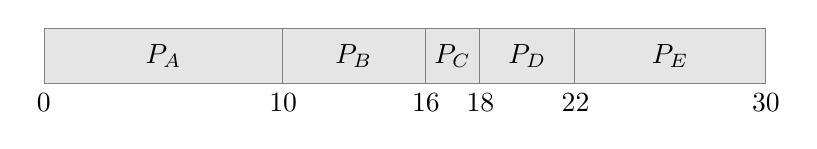
\begin{tikzpicture}[node distance=-0.5pt]
        \node [gray box=10] (p1) {\(P_{A}\)};
        \node [gray box=6, right=of p1] (p2) {\(P_{B}\)};
        \node [gray box=2, right=of p2] (p3) {\(P_{C}\)};
        \node [gray box=4, right=of p3] (p4) {\(P_{D}\)};
        \node [gray box=8, right=of p4] (p5) {\(P_{E}\)};

        \node [annotation] at (p1.south west) {0};
        \node [annotation] at (p1.south east) {10};
        \node [annotation] at (p2.south east) {16};
        \node [annotation] at (p3.south east) {18};
        \node [annotation] at (p4.south east) {22};
        \node [annotation] at (p5.south east) {30};
      \end{tikzpicture}

      \textbf{Average waiting time:} $(0 + \{10 - 0\} + \{16 - 0\} + \{18 - 0\} + \{22 - 0\}) \div 5 = 13.2$ \\
    \end{center}

    \begin{center}
      \smallcaps{(b) Shortest Job First (SJF)}
      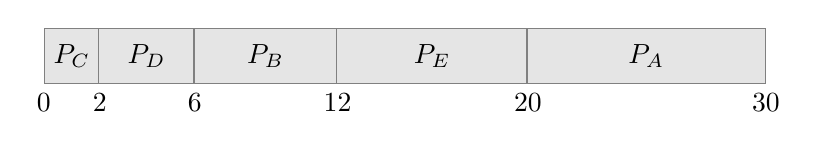
\begin{tikzpicture}[node distance=-0.5pt]
        \node [gray box=2] (p1) {\(P_{C}\)};
        \node [gray box=4, right=of p1] (p2) {\(P_{D}\)};
        \node [gray box=6, right=of p2] (p3) {\(P_{B}\)};
        \node [gray box=8, right=of p3] (p4) {\(P_{E}\)};
        \node [gray box=10, right=of p4] (p5) {\(P_{A}\)};

        \node [annotation] at (p1.south west) {0};
        \node [annotation] at (p1.south east) {2};
        \node [annotation] at (p2.south east) {6};
        \node [annotation] at (p3.south east) {12};
        \node [annotation] at (p4.south east) {20};
        \node [annotation] at (p5.south east) {30};
      \end{tikzpicture}

      \textbf{Average waiting time:} $(\{20 - 0\} + \{6 - 0\} + 0 + \{2 - 0\} + \{12 - 0\}) \div 5 = 8$ \\
    \end{center}

    \begin{center}
      \smallcaps{(c) Longest Job First (SJF)}
      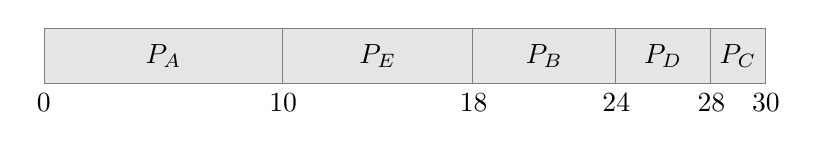
\begin{tikzpicture}[node distance=-0.5pt]
        \node [gray box=10] (p1) {\(P_{A}\)};
        \node [gray box=8, right=of p1] (p2) {\(P_{E}\)};
        \node [gray box=6, right=of p2] (p3) {\(P_{B}\)};
        \node [gray box=4, right=of p3] (p4) {\(P_{D}\)};
        \node [gray box=2, right=of p4] (p5) {\(P_{C}\)};

        \node [annotation] at (p1.south west) {0};
        \node [annotation] at (p1.south east) {10};
        \node [annotation] at (p2.south east) {18};
        \node [annotation] at (p3.south east) {24};
        \node [annotation] at (p4.south east) {28};
        \node [annotation] at (p5.south east) {30};
      \end{tikzpicture}

      \textbf{Average waiting time:} $(0 + \{18 - 0\} + \{28 - 0\} + \{24 - 0\} + \{10 - 0\}) \div 5 = 16$ \\
    \end{center}

    \begin{center}
      \smallcaps{(d) Priority Scheduling $\to$ 3,5,2,1,4}
      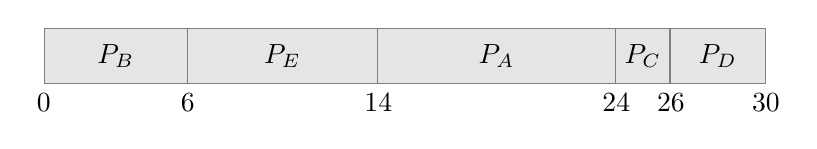
\begin{tikzpicture}[node distance=-0.5pt]
        \node [gray box=6] (p1) {\(P_{B}\)};
        \node [gray box=8, right=of p1] (p2) {\(P_{E}\)};
        \node [gray box=10, right=of p2] (p3) {\(P_{A}\)};
        \node [gray box=2, right=of p3] (p4) {\(P_{C}\)};
        \node [gray box=4, right=of p4] (p5) {\(P_{D}\)};

        \node [annotation] at (p1.south west) {0};
        \node [annotation] at (p1.south east) {6};
        \node [annotation] at (p2.south east) {14};
        \node [annotation] at (p3.south east) {24};
        \node [annotation] at (p4.south east) {26};
        \node [annotation] at (p5.south east) {30};
      \end{tikzpicture}

      \textbf{Average waiting time:} $(\{14 - 0\} + 0 + \{24 - 0\} + \{26 - 0\} + \{6 - 0\}) \div 5 = 14$ \\
    \end{center}

    \pagebreak

    \section*{Synchronization}

    \begin{multicols*}{2}
      \begin{algorithm}[H]
        \While{true}{
          wait(wrt)\;
          \tcp{writing is performed}\label{cmt}
          signal(wrt)\;
        }
      \caption{Reader}
      \end{algorithm}

      \vfill
      \columnbreak

      \begin{algorithm}[H]
        \While{true} {
          wait(mutex)\;
          readCount$++$\;
          \If{readCount == 1} {
            wait(wrt)\;
          }
          signal(wrt)\;
          \tcp{reading is performed}\label{cmt}
          wait(mutex)\;
          readCount$--$\;
          \If{readCount == 0} {
            signal(wrt)\;
          }
          signal(mutex)\;
        }
      \caption{Writer}
      \end{algorithm}
    \end{multicols*}

\end{document}
